\documentclass[../../memoria.tex]{subfiles}

\begin{document}

\paragraph{}
Una vez definida la solución, se va a desarrollar e implementar de manera completa. El primer paso es crear una cuenta en AWS. Al ser una cuenta nueva, permitirá usar la capa gratuita de AWS \cite{awsfreetier}. Esta capa gratuita incluye lo siguiente, entre otros muchos servicios adicionales:

\begin{itemize}
    \item 750h al mes de Elasticsearch Service (instancia tipo t2.small.elasticsearch y una sola zona de disponibilidad) y 10Gb de almacenamiento EBS.
    \item 250K mensajes publicados o enviados al mes para IoT.
    \item 1M de peticiones al mes para AWS Lambda.
\end{itemize}

\paragraph{}
Por tanto, para realizar un \textit{MVP} de la solución, encaja a la perfección.

\paragraph{}
Una vez creada la cuenta en AWS, el siguiente paso es crear un IAM User para Terraform, que tendrá como nombre terraform.

\begin{figure}[H]
    \centering
    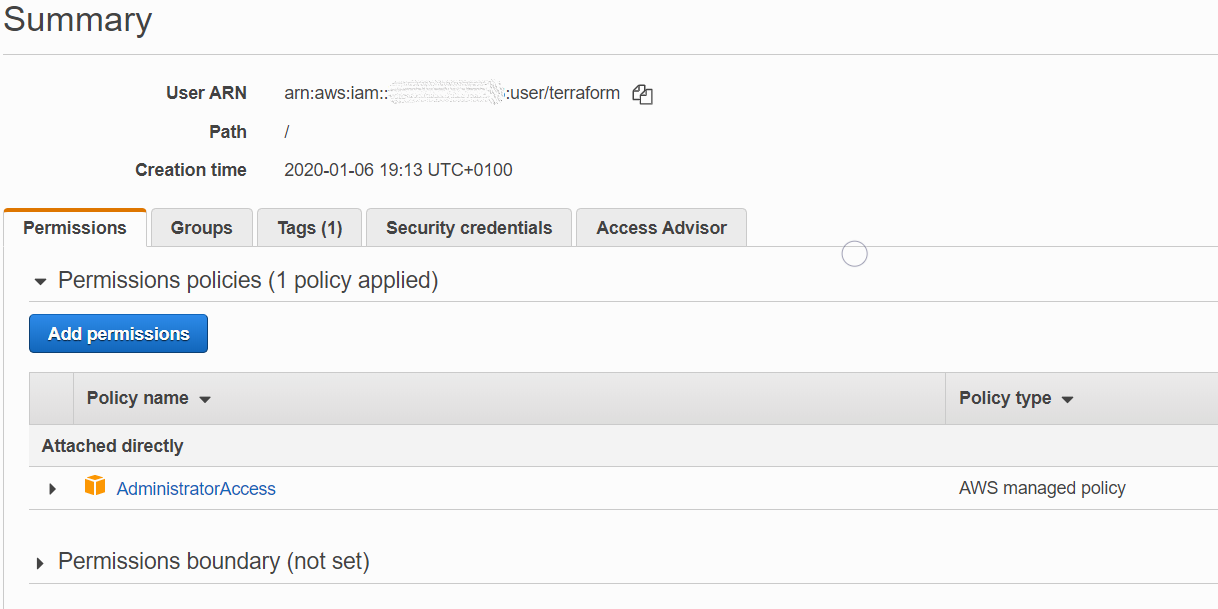
\includegraphics[width=0.7\columnwidth]{figura4.png}
    \caption{Política del usuario Terraform}
    \label{fig:figura4}
\end{figure}

\paragraph{}
Como puede observarse en la Figura 4, el usuario terraform necesita acceso a todos los servicios de AWS. Podría únicamente tener acceso a los servicios para los cuales se vaya a desplegar infraestructura, sin embargo, otorgarle política de administración evitará problemas cuando sea necesario interactuar con otros servicios no contemplados en su política.

\paragraph{}
Asimismo, en la siguiente imagen, la Figura 5, puede observarse que este usuario no cuenta con acceso a la consola web de AWS ya que únicamente necesita acceder de manera programática a través de la API de AWS:

\begin{figure}[H]
    \centering
    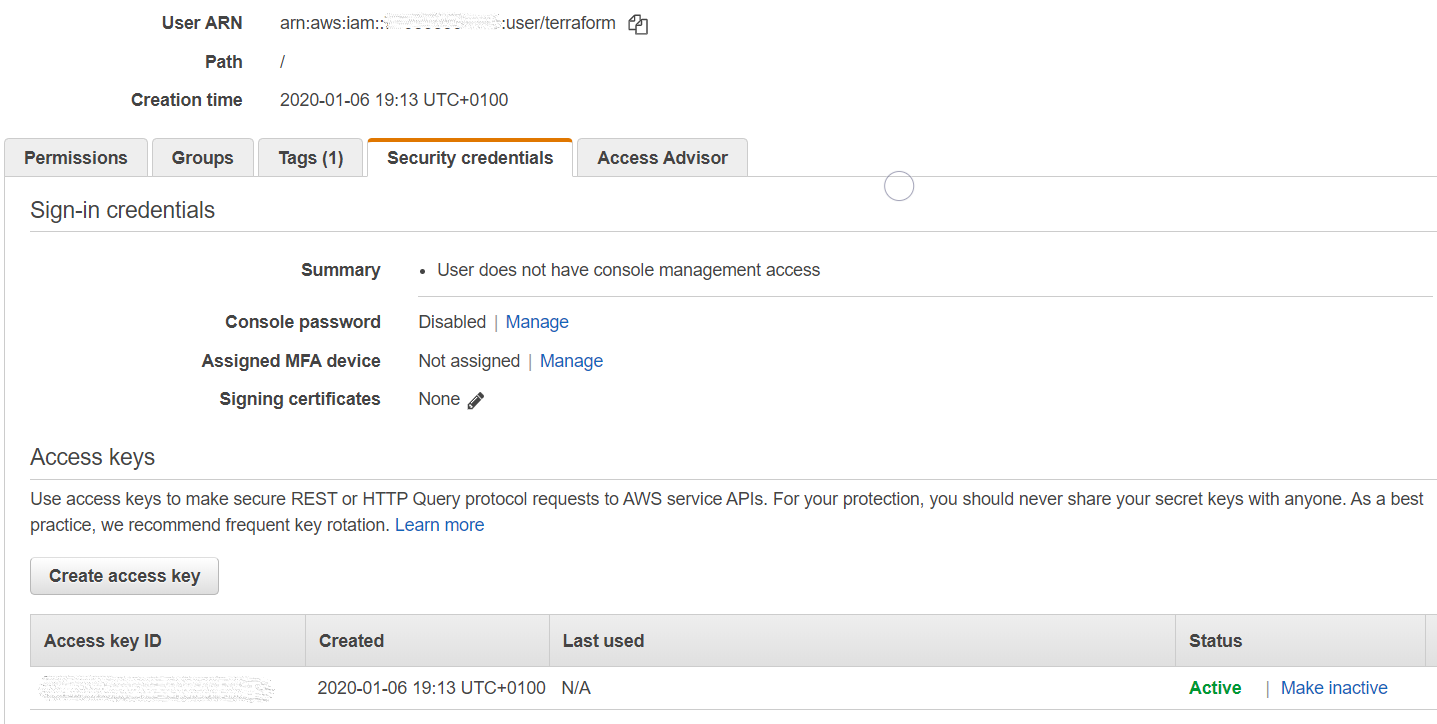
\includegraphics[width=0.7\columnwidth]{figura5.png}
    \caption{Security Credentials en el usuario Terraform}
    \label{fig:figura5}
\end{figure}

\paragraph{}
Como resultado de crear este usuario, AWS genera un \textit{Access Key} y un \textit{Secret Key} que serán las credenciales del usuario terraform, y que será necesario, de cualquiera de los métodos posibles, entregárselas al programa Terraform para realizar los despliegues de la infraestructura.

\end{document}
